 \documentclass[11pt]{article}

\usepackage[T1]{fontenc}
\usepackage[sc]{mathpazo}

%%%%%%%%%%%%%%%%%%%%%%%%%%%%%%%
% 
% Header: Please do not modify  !!!!
% (see below if you need to add some \newcommand)
%%%%%%%%%%%%%%%%%%%%%%%%%%%%%%%%

%%%%%%%%%%%%%%%%%%%%%%%%%%%%%%%
% Beginning: appearance
\usepackage[includefoot]{geometry}
\geometry{paperwidth=7in, paperheight=10.5in, vmargin=0.6in, inner=0.75in, outer=0.5in}
\setlength{\parindent}{0pt}
\setlength{\parskip}{2ex}
\pagestyle{plain}
% ----------- End: appearance
%%%%%%%%%%%%%%%%%%%%%%%%%%%%%%%%

%%%%%%%%%%%%%%%%%%%%%%%%%%%%%%%
% Beginning: ams
\usepackage{amsmath}
\usepackage{amssymb}
\usepackage{amsthm}
\usepackage{array}
% ----------- End: ams
%%%%%%%%%%%%%%%%%%%%%%%%%%%%%%%%

%%%%%%%%%%%%%%%%%%%%%%%%%%%%%%%
% Beginning: tikz libraries
\usepackage{tikz}
\usepackage{tikz-3dplot}
\usepackage{pgfplots}
\pgfplotsset{compat=1.15}
%\usepackage{tkz-graph}
\usetikzlibrary{arrows}
\usetikzlibrary{arrows.meta}
\usetikzlibrary{automata}
\usetikzlibrary{decorations.markings}
\usetikzlibrary{patterns}
\usetikzlibrary{positioning}
\usetikzlibrary{shapes.geometric}
% ----------- End: Theorems, Definitions
%%%%%%%%%%%%%%%%%%%%%%%%%%%%%%%%

%%%%%%%%%%%%%%%%%%%%%%%%%%%%%%%
% Beginning: misc.
\usepackage{pdfpages}

\usepackage{pifont}
\usepackage{forest}

\usepackage{multirow,multicol,enumitem}

\usepackage{ytableau}
\usepackage{bm}
\usepackage{bbm}

\usepackage{caption}
\usepackage{mathrsfs}
% ----------- End: misc.
%%%%%%%%%%%%%%%%%%%%%%%%%%%%%%%%

%%%%%%%%%%%%%%%%%%%%%%%%%%%%%%%
% Beginning: Theorems, Definitions,
\theoremstyle{plain}
\newtheorem{theorem}{Theorem}
\newtheorem{corollary}[theorem]{Corollary}
\newtheorem{lemma}[theorem]{Lemma}
\newtheorem{proposition}[theorem]{Proposition}
\newtheorem{conjecture}[theorem]{Conjecture}
\newtheorem{question}[theorem]{Question}
%
\theoremstyle{definition}
\newtheorem{definition}[theorem]{Definition}
\newtheorem{example}[theorem]{Example}
%
\theoremstyle{remark}
\newtheorem{remark}[theorem]{Remark}
% ----------- End: Theorems, Definitions
%%%%%%%%%%%%%%%%%%%%%%%%%%%%%%%%
% Beginning: Custom title/name etc entries
\usepackage{titlesec}
\titleformat{\section}{\Large\sc\linespread{0.75}\selectfont\hyphenchar\font=-1\relax}{}{0em}%
{}[\vspace{-8pt}\rule{1.0\textwidth}{1pt}\vspace{-10pt}]
\titleformat{\subsection}{\large\bf}{}{0em}{}
\titlespacing{\section}{0em}{2em}{0em}

\newcommand{\name}[1]{\noindent {\it #1}\medskip}
\newcommand{\adr}[1]{\hfill {#1}}
\newcommand{\jointwork}[1]{\noindent {\it This talk is based on joint work with #1}\medskip}
% ----------- End: Custom title/name etc entries
%%%%%%%%%%%%%%%%%%%%%%%%%%%%%%%
% 
% End of the Header
%
%%%%%%%%%%%%%%%%%%%%%%%%%%%%%%%%

%%%%%%%%%%%%%%%%%%%%%%%%%%%%%%%%%%%%%%%%%%%%%%%%%%%%%%%%%%%%%%%%%%%%%%%%%%%%%%%%%%%%%%%%%%%%%%%%%%%%

%%%%%%%%%%%%%%%%%%%%%%%%%%%%%%%
% Beginning: Your own \newcommand
% !!!!!!!!!
% Put here your personal commands
% !!!!!!!!!
\newcommand{\essence}{\texttt{Essence} }
\newcommand{\conjure}{\texttt{Conjure} }
\usepackage{listings}
\lstset{
%basicstyle=\footnotesize\ttfamily,
basicstyle=\scriptsize\ttfamily,
mathescape,
numbers=none,
keywordstyle=\bfseries, %\color{red}
keywords = {language, Essence, given, letting, find, such, that,
bool, int, matrix, enum, variant, record, set, mset,
sequence, function, relation, partition,
domain, total, surjective, be,
forAll, exists, sum, injective, in, preImage, range,
new, type, intersect, union, from,
minimising, maximising, of, indexed, by, and, or, toInt, numParts, partSize, together,
defined, maxSize, maxNumParts, size, regular, language, cheese
}
showstringspaces=false,
tabsize=1,
breaklines=true,
breakatwhitespace=false
}
% ----------- End: Your own \newcommand
%%%%%%%%%%%%%%%%%%%%%%%%%%%%%%%%


\begin{document}

% Title of the contribution:
\section*{Using Constraint Programming to Enumerate Permutations avoiding Mesh Patterns}
% Author:
  \name{Ruth Hoffmann}
    \adr{University of St Andrews}

% Co-authors:
\jointwork{\"{O}zg\"{u}r Akg\"{u}n, Chris Jefferson}

% Short description

Constraint programming is a proven technology for solving complex combinatorial decision, optimisation or enumeration problems. 
Constraints are a natural, powerful means of representing and reasoning about complex problems that impact all of our lives.
Constraint programming offers a means by which solutions to such problems can be found automatically, and proceeds in two phases. 
First, the problem is modelled as a set of decision variables, and a set of constraints on those variables that a solution must satisfy. 
A decision variable represents a choice that must be made in order to solve the problem. 
The domain of potential values associated with each decision variable corresponds to the options for that choice.

Enumerating permutations avoiding mesh (or other) patterns lends itself perfectly to constraint programming.
We have created a model which represents the definition of a mesh pattern \cite{branden2011mesh} in \essence \cite{essence}. 
We then use \conjure \cite{conjure} to solve a range of permutation pattern problems. 
We can find if a pattern is present inside a target permutation at all, or count how many permutations of a certain length (or range of lengths) avoid the pattern or a set of patterns.

\essence is a high-level problem specification language: it natively supports decision variables with abstract domains like set, multi-set, function, relation, partition domains and operations defined on these domains. 
\conjure translates problem specifications into concrete models suitable as input to standard constraint programming toolkits.
\conjure allows practitioners to explore alternative approaches to convert problem specifications to concrete models and allows the use of different state-of-the-art black box solvers. 
The solver that we use in this work are Minion\cite{minion} and an AllSAT solver \texttt{nbc\_minisat\_all} \cite{nbcminisatall}.

The main benefit of modelling permutation patterns as a set of constraints is that constraint models are highly modular.
This means it is easy to use the same (or only slightly modified) code to find the permutations which satisfy a set of patterns, or find permutations which contain one mesh pattern, but do not contain a second mesh pattern.

\begin{figure}
\begin{lstlisting}[numbers=left,escapechar=£]
language Essence 1.3

given avoid : set of (sequence(injective) of int, relation of (int*int)) £\label{line:mesh}£

given n : int
find perm : matrix indexed by [int(0..n+1)] of int(0..n+1) £\label{line:permstart}£

such that
  perm[0] = 0, perm[n+1] = n+1,
  allDiff(perm) £\label{line:permend}£
    
such that
  forAll (av, mesh) in avoid .
  exists avinv: matrix [int(0..|av|+1)] of int(0..|av|+1),£\label{line:avinvs}£
    and([avinv[0] = 0, avinv[|av|+1] = |av|+1,
         (forAll i: int(1..|av|) . avinv[av(i)] = i)]. £\label{line:avinve}£
      forAll ix : matrix indexed by [int(0..|av|+1)] of int(0..n+1),£\label{line:ixs}£
        and([ ix[0]=0 /\ ix[|av|+1]=n+1
            , forAll i : int(0..|av|) . ix[i] < ix[i+1]
            , forAll n1, n2 : int(1..|av|) , n1 < n2 .
                av(n1) < av(n2) <-> perm[ix[n1]] < perm[ix[n2]]£\label{line:ixe}£
            ]) .
          ( exists i,j: int(0..|av|). £\label{line:meshs}£
            (i,j) in mesh /\
            exists z: int(ix[i]+1..ix[i+1]-1).
              (perm[ix[avinv[j]]] <= perm[z] /\ perm[z] <= perm[ix[avinv[j+1]]])
          ) £\label{line:meshe}£
\end{lstlisting}
\caption{The \essence specification of the mesh pattern avoidance. \label{fig:model}}
\end{figure}



\section{Modelling Mesh Patterns}

We will present our model for finding all permutations in $S_n$ which avoid a set of mesh patterns (code in Figure~\ref{fig:model}. 
This model can easily be extended to consider many similar problems. 
Our models are given in \essence, a high-level constraint modelling language. 

\newpage

One of the most difficult part of modelling mesh patterns is edge conditions. 
The cells in the mesh which are around the edge and represent ``all other values''. 
We want to avoid having to handle these values specially. 
To avoid having to special case the edges of the mesh, we extend the permutation \texttt{perm} we search for from a permutation \(p\) in $S_n$ to a permutation on \(\{0,\dots,n+1\}\), where \(0^p=0\) and \((n+1)^p=n+1\) (Lines \ref{line:permstart}--\ref{line:permend}).

The mesh pattern is stored as a set of pairs \texttt{(av, mesh)} (Line \ref{line:mesh}), where \texttt{av} is an injective sequence (representing the permutation) and \texttt{mesh} is a relation representing the cells in the mesh which cannot contain values.
The mesh pattern is defined in a separate file which represents the given information, alongside \texttt{n} which represents the length of target permutations in $S_n$. 
An example file of a mesh pattern is found in Figure~\ref{fig:param}, which represents the mesh pattern in Figure~\ref{fig:pattern}.

We dynamically calculate \texttt{avinv}, the inverse of \texttt{av}. 
Similarly to the permutation, we extend this with an extra value, where \texttt{avinv[0]=0} and \texttt{avinv[x+1] = n+1} (where \texttt{x} is the length of the pattern \texttt{av}) (Lines \ref{line:avinvs}--\ref{line:avinve}). 

We then search for all occurrences of the pattern in the permutation (Lines \ref{line:ixs}--\ref{line:ixe}. 
Similarly when searching for the pattern in a permutation, we add an extra fixed value to the start and end of the pattern, which map to \(0\) and \(n+1\) respectively.

Finally, when we find an occurrence of the pattern, we check that at least one member of the mesh contains a value (which means the mesh is not actually present) (Lines \ref{line:meshs}--\ref{line:meshe}).

We will talk about the model, give more insights into how it and the solving of it works. 
We will present results to show how competitive using a general purpose declarative method (constraint programming) can be in comparison to bespoke algorithms when solving NP-complete enumeration problems and specifically when enumeration mesh pattern avoiding permutations.


\begin{figure}
 \begin{lstlisting}[numbers=left]
language Essence 1.3

letting n be 4

letting avoid be {(sequence(1,3,2), relation((1,2),(2,3),(3,0),(3,1)))}
    
\end{lstlisting}
\caption{The \essence parameter file of a particular mesh pattern and the length of permutations that will be enumerated.\label{fig:param}}
\end{figure}

\begin{figure}
\begin{center}
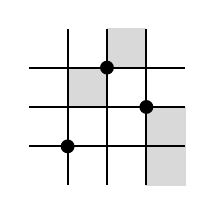
\begin{tikzpicture}[scale=0.5]
    \fill[gray!30] (1,2) rectangle (2,3);
    \fill[gray!30] (2,3) rectangle (3,4);
    \fill[gray!30] (3,0) rectangle (4,1);
    \fill[gray!30] (3,1) rectangle (4,2);
    \draw[line width=0.7pt] (0.01,0.01) grid (3.99,3.99);
    \fill (1,1) circle (5pt);
    \fill (2,3) circle (5pt);
    \fill (3,2) circle (5pt);

\end{tikzpicture}
\caption{Mesh pattern as defined in the parameter file.\label{fig:pattern}}
\end{center}
\end{figure}



\begin{thebibliography}{99}
\bibitem{branden2011mesh} Petter Br{\"a}nd{\'e}n and Anders Claesson. \emph{Mesh patterns and the expansion of permutation statistics as sums of permutation patterns}, Electron. J. Combin. 18(2) (2011).
\bibitem{conjure} Ozgur Akgun, Ian Miguel, Chris Jefferson, Alan M. Frisch, and Brahim Hnich. \emph{Extensible automated constraint modelling}, AAAI (2011).

\bibitem{essence} Alan M. Frisch, Matthew Grum, Chris Jefferson, Bernadette M. Hernández, and Ian Miguel. \emph{The Essence of Essence}, Modelling and Reformulating Constraint Satisfaction Problems 73 (2005).

\bibitem{minion} Chris Jefferson, Ian P. Gent, and Ian Miguel. \emph{Minion: A fast, scalable, constraint solver}, ECAI (2006).

\bibitem{nbcminisatall} Takahisa Toda and Takehide Soh. \emph{Implementing efficient all solutions SAT solvers}, JEA 21 (2016). 

\end{thebibliography}

\end{document}  
